\noindent
\begin{minipage}[t]{0.29\textwidth}
  \vspace{0pt}
  \href{https://visdyn.github.io/TRACE/}{%
    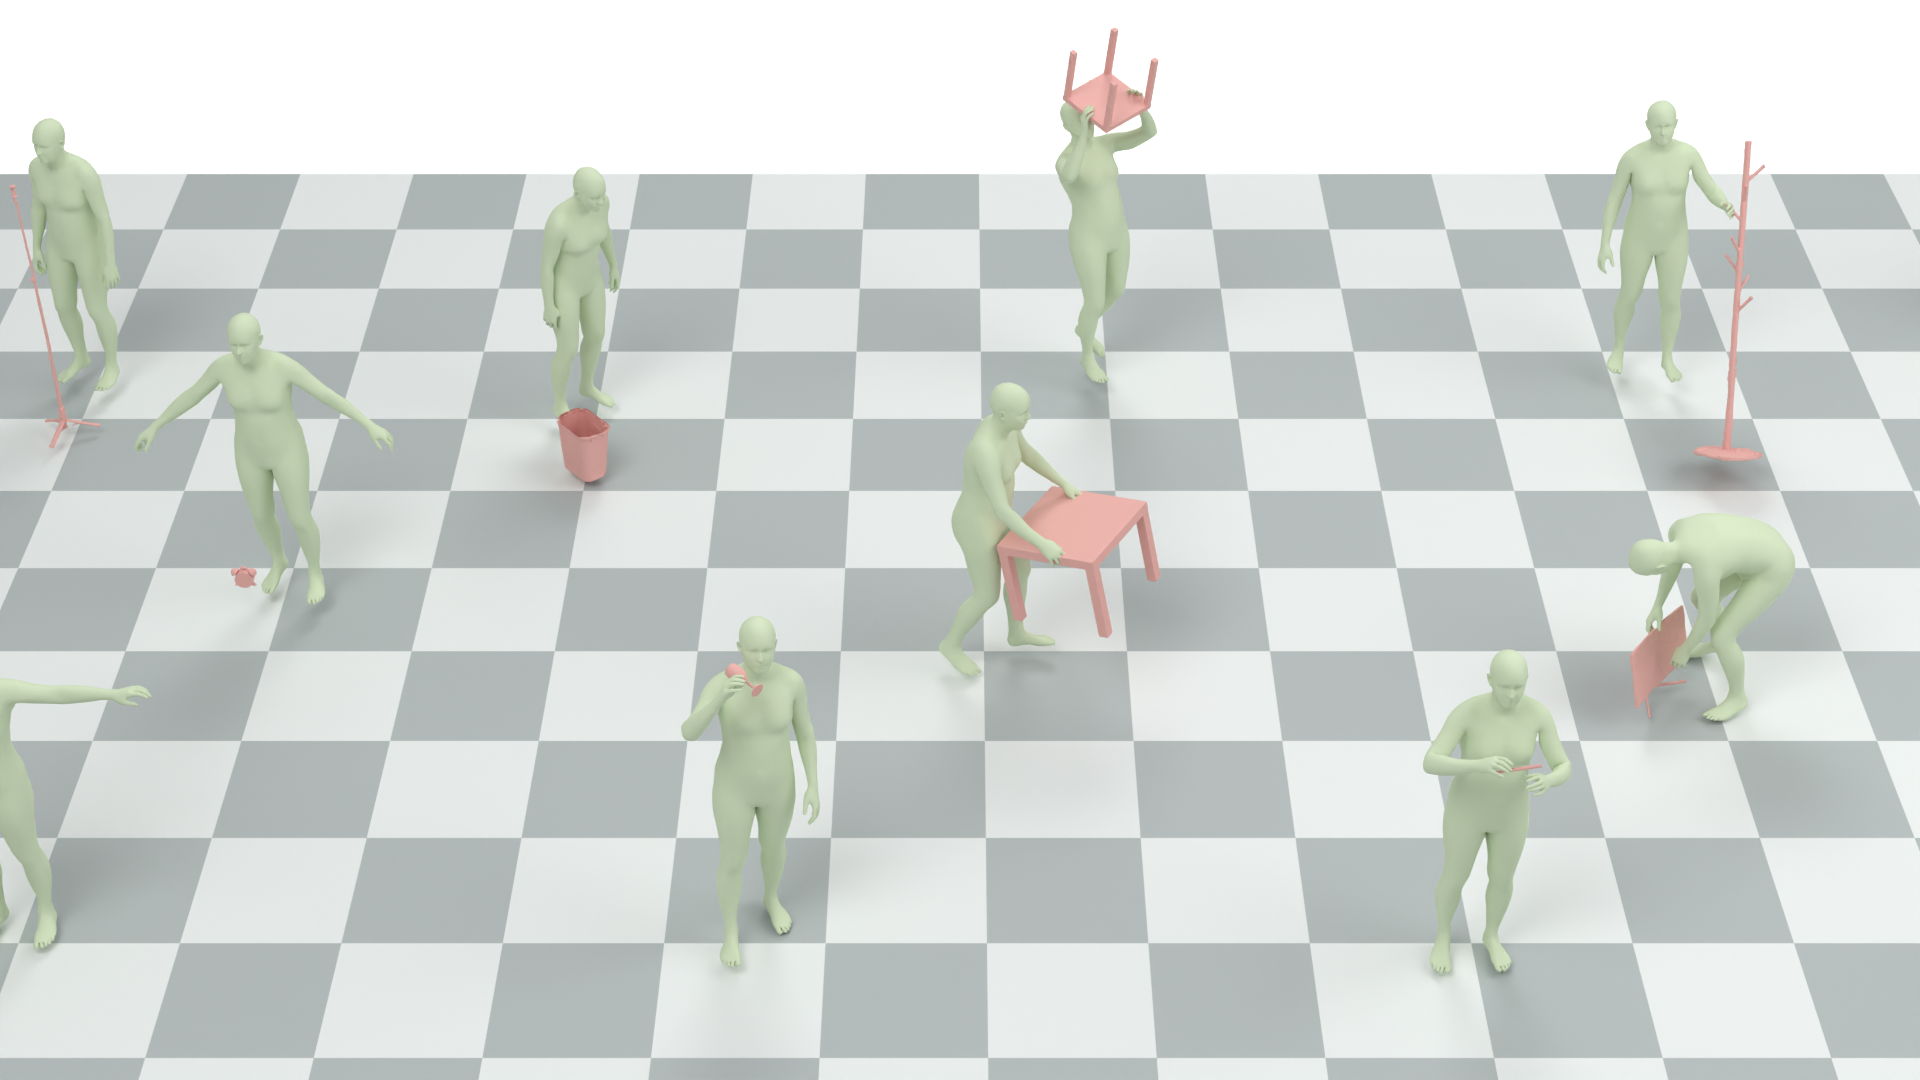
\includegraphics[width=\linewidth,height=1.12in,keepaspectratio]{images/trace-poster.png}}
  \par\vspace{2pt}
  \centering\scriptsize\href{https://visdyn.github.io/TRACE/}{View TRACE demo}
\end{minipage}\hfill
\begin{minipage}[t]{0.68\textwidth}
  \vspace{0pt}
  \hyphenpenalty=10000\exhyphenpenalty=10000
  \noindent\textbf{[1] \href{https://arxiv.org/abs/2609.32551}{Harnessing Coupled Stream Completion for Human-Object Interaction Modeling}}
  \hfill\textit{arXiv, 2026}\par
  \textbf{Dawei Guan}, Di Yang, and Jiangtao Wang\par
  \href{https://arxiv.org/abs/2609.32551}{Paper}
  \enspace | \enspace \href{https://visdyn.github.io/TRACE/}{Project and demo}\par
  TRACE represents body, object, and hand motion in separate latent streams while predicting updates from the complete interaction state. Geometry-aware losses constrain contact, relative pose, and timing after decoding. The framework supports completion of any missing stream and language-model-based interaction understanding.
\end{minipage}

\vspace{0.18in}
\noindent
\begin{minipage}[t]{0.29\textwidth}
  \vspace{0pt}
  \href{https://visdyn.github.io/flowcomotion/}{%
    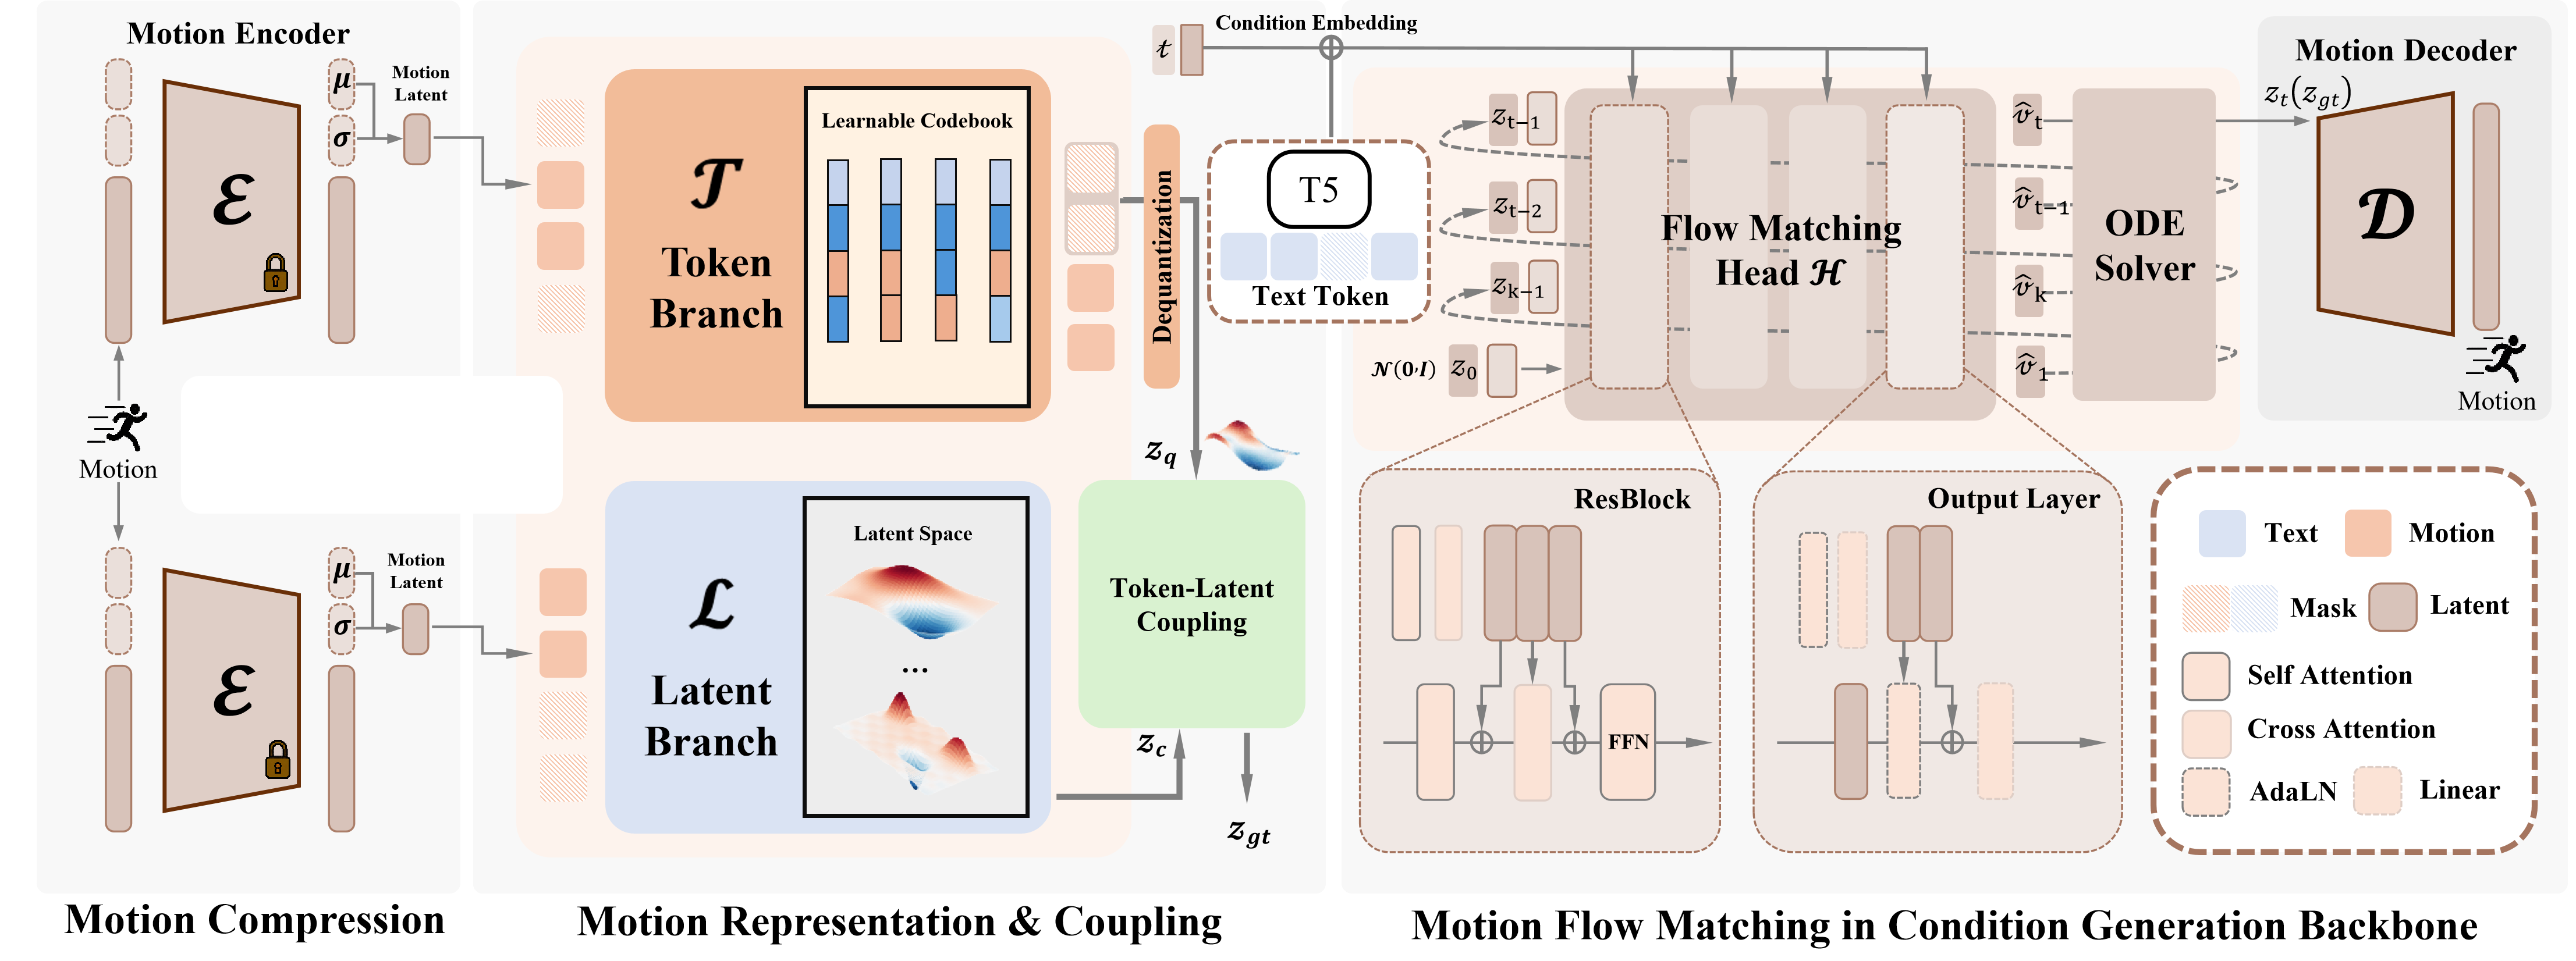
\includegraphics[width=\linewidth,height=1.12in,keepaspectratio]{images/flowcomotion.png}}
  \par\vspace{2pt}
  \centering\scriptsize\href{https://visdyn.github.io/flowcomotion/}{View project demo}
\end{minipage}\hfill
\begin{minipage}[t]{0.68\textwidth}
  \vspace{0pt}
  \hyphenpenalty=10000\exhyphenpenalty=10000
  \noindent\textbf{[2] \href{https://arxiv.org/abs/2604.11083}{FlowCoMotion: Text-to-Motion Generation via Token-Latent Flow Modeling}}
  \hfill\textit{arXiv, 2026}\par
  \textbf{Dawei Guan}, Di Yang, Chengjie Jin, and Jiangtao Wang\par
  \href{https://arxiv.org/abs/2604.11083}{Paper}
  \enspace | \enspace \href{https://visdyn.github.io/flowcomotion/}{Project and demo}\par
  FlowCoMotion combines discrete motion tokens with continuous latents to retain semantic structure and fine motion detail. Multi-view distillation regularizes the continuous space, while temporal quantization extracts semantic cues. A text-conditioned velocity field is integrated with an ODE solver to generate motion.
\end{minipage}
\par\vspace{0.1in}
